\subsection{ETMailFilter}

É um filtro de \emph{email} que permite definir, por utilizador, um conjunto de domínios e/ou endereços de \emph{email} dos quais o utilizador pode ou não receber mensagens.
Permite também filtrar os \emph{emails} com base no seu conteúdo dos anexos. Esta filtragem pode ser feita com base na extensão dos ficheiros em anexo e/ou com base no seu \emph{MIME Type}.

O fluxo das mensagens é descrito na Figura \ref{fig:etmf}.

\begin{figure}[p]
\centering
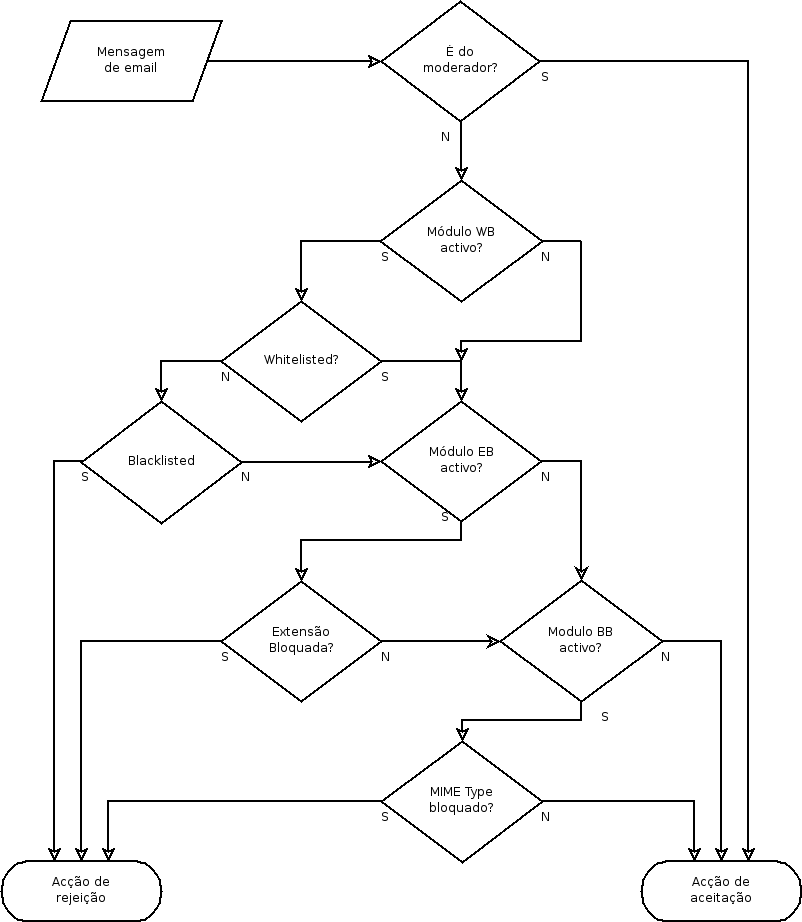
\includegraphics[width=\textwidth]{include/img/etmf}
\caption{Fluxo das mensagens de email}
\label{fig:etmf}
\end{figure}

